\documentclass[12pt,a4paper]{article}
\usepackage{hyperref}
\usepackage{graphicx}
\usepackage{epstopdf}
\usepackage[section]{placeins}
\usepackage{array}
\usepackage{amsmath}

\title{Finding Optimized Machine Learning Model For Recognizing English Handwritten Digit}
\author{Nowfel Mashnoor\\Roll: 1503069\and Amir Faruk\\Roll: 1503075}

\begin{document}
\date{}
\maketitle

\begin{abstract}
This paper is about the comparison between different Machine Learning models(classifiers) trained and tested on MNIST dataset. For declaring a model as best, we only considered low error score. A standard machine learning library written in Python Programming Language is used during this research. 
\end{abstract}

\section{Introduction}
Handwritten Digit Recognition has been very successful in recent years. A lot of research and studies has been done in recent years on it like Devnagari Handwritten Character Recognition\cite{pal2009comparative}. Handwritten digit recognition technique is used in various fields like PDA, bank cheque, handwritten fields in form etc.\cite{plamondon2000online} Using machine learning technique, which which can be briefly defined as enabling computers make successful predictions using past experiences, \cite{bacstanlar2014introduction} handwritten digit recognition system is greatly improved. Handwritten Digit recognition is a supervised learning algorithm problem. There are many classifier in supervised learning like Neural Network, Decision Tree,  Bayesian Network, Support Vector Machine(SVM), Random Forest etc\cite{kotsiantis2007supervised}. A comparison study has been already done where \textit{Base Linear Classifier, Baseline Nearest Neighbor Classifier, Large Fully Connected Multi-Layer Neural Network, Tangent Distance Clasifier(TDC), LeNet 4 With KNN, Optimal Margin Classifier} are compared among.\cite{lecun1995learning} In our research we are going to compare among Random Forest and Artificial Neural Network. We will chose the best classifier among them based on their accuracy on testing set. 

\section{MNIST Dataset}

For training and testing our classifiers, we used MNIST (Modified National Institute of Standards and Technology) Dataset. This dataset contains \textit{70000} images. Among 70000 images, 60000 images are for training and 10000 images are for testing\cite{kussul2004improved}.  It is basically a subset of NIST dataset. the black and white images from NIST were normalized to fit into a 28x28 pixel and converter to grayscale levels.\cite{lecuncourant}

\begin{figure}[!htb]
  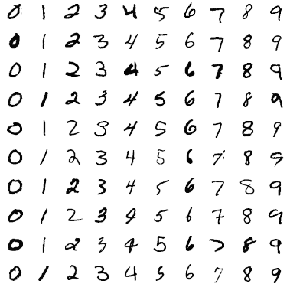
\includegraphics[width=5cm,height=5cm,keepaspectratio]{mnist_example.png}
  \centering
  \caption{MNIST Dataset Sample Images}
  \label{fig:mnist_sample}
\end{figure}
For each and every classifier we are using in our study, we will use use all the 60000 images for training and the rest 10000 images for evaluating our models. 

\section{Scikit Learn Machine Learning Library}
Scikit-learn is a Python module integrating a wide range of state-of-the-art machine learning algorithms for medium-scale supervised and unsupervised problems\cite{pedregosa2011scikit}. Most of the algorithms are written in Python programming language where some of the algorithms are written in Cython for achieving optimal performance. Also for efficient operation on large arrays and multidimensional matrices, we used NumPy library.\cite{walt2011numpy} For graphing and other visualization purpose, we used Matplotlib, which is other Python Library. \cite{hackeling2014mastering} For training and testing our classifiers, we will use the Scikit Learn Library. This library also provides tools for model evaluation. 


\section{The Classifiers}
We have trained and tested three classifiers on MNIST Dataset. We are going to give a quick and brief description of all of them. 
\subsection{Random Forest}
Random Forest is a powerful Machine Learning model. It can do both regression and classification.\cite{liaw2002classification} It is basically a collection of random decision trees. Each decision tree predict a class and after all the prediction, random forest outputs that class which got the most vote. The main benefit of Random Forest over decision tree is that it removes the problem of over fitting of decision tree.\cite{friedman2001elements} 
\begin{figure}[!htb]
  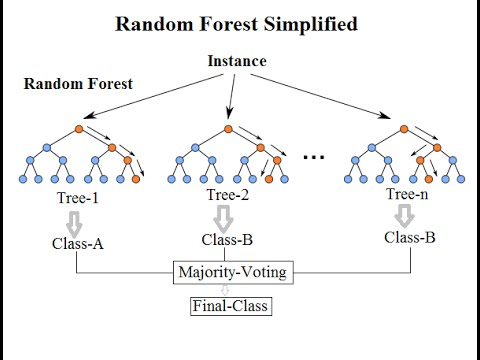
\includegraphics[width=10cm,height=10cm,keepaspectratio]{random_forest.jpg}
  \centering
  \caption{Random Forest}
  \label{fig:random_forest}
\end{figure}
Random forest uses Bootstrap aggregating or Tree Bagging algorithm. It reduces variance and helps to prevent over fitting. In decision tree learning, for splitting the variable at each step, different metrics can be used like Gini Impurity, Information Gain. We used Gini Index or Gini Impurity in our work. For calculating Gini Index, we have to use the following formula: \\
\centerline{$I_{G}(P)$ = $\sum_{i=1}^{J}p_{i}\sum_{k\neq{i}}p_{k}$}
Where,\\
J = No. of Classes\\
i $\epsilon$ {1, 2, 3, ..., J}\\
$p_{i}$ = Probability of an item with label \textit{i} being chose\\
$p_{k}$ = Probability of a mistake categorizing that item \cite{wiki:decisiontreelearning}
 
\subsection{Artificial Neural Network}
Artificial Neural Network(ANN) is a computing system inspired by biological neural network that constitute animal brains.\cite{vangerven2017artificial} It is one of the best models for both classification and regression. Generally Neural Networks learns from example. It is given some training set and from that training set, it generates a set of weight vectors. This training is can be done using various learning algorithm. In our work, we have use backpropagation algorithm which is a popular method for designing a multi layer neural network.\cite{leung1991complex} A Neural Network system has some layer. Each layer contains some neurons. The first layer is called input layer and the last layer is called output layer. The other layers that lies in between is called hidden layers. Each neuron is given a vector from previous layer as input and then it passes the value to a non-linear transfer function and generates a input for the next layer.\cite{hagan1996neural} 
\begin{figure}[!htb]
  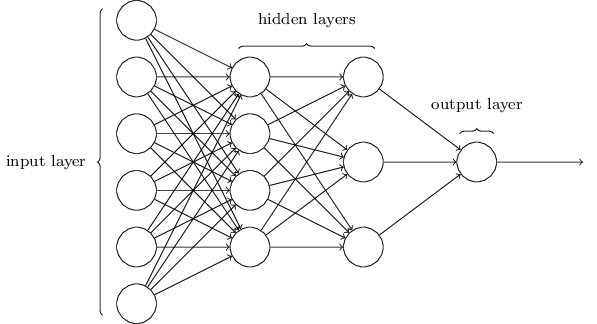
\includegraphics[width=10cm,height=10cm,keepaspectratio]{neuralnet.png}
  \centering
  \caption{Neural Network}
  \label{fig:NeuralNet}
\end{figure}
The transfer function, by which the neuron takes input and gives a output is also called activation function. There are many activation functions like Logistic or Sigmoid, Softsign\cite{bergstra2009quadratic}, Inverse square root unit\cite{carlile2017improving}, rectified linear unit(ReLU)\cite{hinton2010rectified}, Exponential Linear Unit (ELU)\cite{clevert2015fast} In our work we have used Sigmoid as transfer function. Also used backpropagation algorithm as it is capable of handling large problems.\cite{hecht1992theory}  
\section{Hyperparameters}
Hyperparamters basically are the tuning knobs of a learning algorithm. There parameters are set before the training of the machine learning model.\cite{wiki:Hyperparameter} By changing the parameters, we can tune the model.\cite{hutter2014efficient} After many trial and error, we have set these hyper parameter values.
\subsection{For Random Forest}
\textit{The number of trees in the forest = 10}\\
\textit{criterion = gini}\\
\textit{Minimum samples split = 2}\\
\textit{Minimum Samples Leaf = 1}\\
\textit{Min Weight Fraction Leaf = 0}\\
\textit{min impurity decrease = 0}\\
\textit{The number of jobs to run in parallel for both fit and predict = 2}
\subsection{Artificial Neural Network}
\textit{Hidden Layer Size = 30, 30, 30}\\
\textit{Activation = Logistic(Sigmoid)}\\
\textit{The Solver for Weight Optimization = stochastic gradient descent}\\
\textit{Learning Rate = 0.001}\\
\textit{Tolerance = 1e-4}
\section{Model Evaluations}
After testing the model, we have tested all our classifiers using the test dataset of MNIST. The following tables will show our findings on this test. We not only calculated the error rate of the model, but also Mean Accuracy, F1 Score, Recall Score and Confusion matrix.
\subsection{Precision Score}
\begin{center}
\begin{tabular}{ || c c c c c c c|| } 
\hline
Classifier & Cls 0 & Cls 1 & Cls 2 & Cls 3 & Cls 4 & Cls 5\\
 \hline
 RF & 0.95829196 & 0.97650131 & 0.92701422 & 0.92625369 & 0.95829095 & 0.94557823\\ 
\hline
ANN & 0.93841336 & 0.94482759 & 0.80925401 & 0.8387698 & 0.89559877 & 0.80462725\\
 \hline
\end{tabular}
\end{center}


\begin{center}
\begin{tabular}{ || c c c c c c || } 
\hline
Classifier & Cls 6 & Cls 7 & Cls 8 & Cls 8 & Cls 9\\
 \hline
 RF & 0.95829196 & 0.97650131 & 0.92701422 & 0.92625369 & 0.95829095\\ 
\hline
ANN & 0.93841336 & 0.94482759 & 0.80925401 & 0.8387698 & 0.89559877\\
 \hline
\end{tabular}
\end{center}

\subsection{Average Accuracy}
\begin{center}
\begin{tabular}{ || c c || } 
\hline
Artificial Neural Netwrok & Random Forest\\
\hline
0.875087508750875 & 0.9478947894789479\\
 \hline
\end{tabular}
\end{center}

\subsection{F1 Score}
\begin{center}
\begin{tabular}{ || c c c c c c c|| } 
\hline
Classifier & Cls 0 & Cls 1 & Cls 2 & Cls 3 & Cls 4 & Cls 5\\
 \hline
 RF & 0.96203796 & 0.98380744 & 0.93937947 & 0.9286066 & 0.94977169 & 0.92699491\\ 
\hline
ANN & 0.92823955 & 0.95511983 & 0.81970349 & 0.86413826 & 0.89331291 & 0.7497006\\
 \hline
\end{tabular}
\end{center}

\begin{center}
\begin{tabular}{ || c c c c  c || } 
\hline
Classifier & Cls 6 & Cls 7 & Cls 8  & Cls 9\\
 \hline
 RF & 0.96675462 & 0.95022178 & 0.93067227 & 0.9341258\\ 
\hline
ANN & 0.92169312 & 0.91530461 & 0.84148728 & 0.83781095\\
 \hline
\end{tabular}
\end{center}

\subsection{Recall Score}
\begin{center}
\begin{tabular}{ || c c c c c c c|| } 
\hline
Classifier & Cls 0 & Cls 1 & Cls 2 & Cls 3 & Cls 4 & Cls 5\\
 \hline
 RF & 0.98365679 & 0.99030837 & 0.95348837 & 0.93366337 & 0.95315682 &  0.91816143\\ 
\hline
ANN & 0.91828396 & 0.96563877 & 0.83042636 & 0.89108911 & 0.8910387 & 0.70179372\\
 \hline
\end{tabular}
\end{center}
\subsection{Confusion Matrices}
\subsubsection{For Random Forest}

\[
CM=
  \begin{bmatrix}
   965  &  0 &   1   & 1   & 1  &  2  &  3  &  1  &  5  &  0\\
0 & 1118  &  3  &  2  &  1   & 2  &  2  &  1 &   6 &   0\\
6  &  4 & 984 &   6  &  6  &  1  &  4 &  12  &  5  &  4\\
1  &  3  &  11  &  958  &  1  &  13  &  0  &  7 &   10  &   6\\
5  &   2 &   4  &  0 &  937 &   2 &   4  &  4 &   5 &  19\\
6   &  1  &   2  &  26  &  5  &  836  &  4   &  1  &   4 &   7\\
12  &  6  &  0 &   0  &  4 &  11 &  920  &   1  &  4  &  0\\
5   &  6 &  25  &   9  &  4  &  0  &  0 & 962  &  3 &  14\\
14  &  1 &  13 &  29 &  10 &  21 &   8 &   6 & 863 &    9
  \end{bmatrix}
\]

\subsubsection{For Artificial Neural Network}
\[
CM=
  \begin{bmatrix}
899  &  0  & 43  &  2  &  0 &  23  &  8  &  1  &  2  &  1\\
0 & 1096  &  2 &   2  &  0  &  1 &   1  &  1 &  30  &  2\\
13  &  3 & 857  &  3  &  8  & 43  & 25 &   7 &  53 &  20\\
1 &   5  &  9 & 900  &  0  & 55  &  0 &   7 &  33 &   0\\
0  &  0 &  10 &   0 & 875  &  0  & 19  &  4 &   5 &  69\\
21  &  4  & 52 & 142  &  0 & 626  &  5 &   0  & 38 &   4\\
18 &   1  & 38 &   0 &  20  &  3 & 871  &  0 &   5   & 2\\
1 &  31 &   3  &  1 &   2 &   0  &  1 & 924 &  19 &  46\\
4 &  14 &  37 &  18  &  6 &  13  &  0  &  7 & 860 &  15\\
1  &  6 &   8  &  5  &  66 &  14 &   2 &  40 &  25 & 842
  \end{bmatrix}
\]
\subsection{Overall Running Time}
Random Forest = \textit{2.2805209159851074 s}\\
ANN = \textit{82.07250833511353 s}\\\\
\textbf{Hardware Specification}\\\\
Processor: Intel Corei7\\
Speed: 3.5GHz\\
RAM: 16 GiB DDR3\\
OS: macOS High Sierra


\section{Discussion}
From the above scores, it's clear that Random forest is showing much greater performance than the Artificifial Neural Network in this case. The average accuracy on MNIST Test Data Set, which is considered as one of the most vital factor of a model, is quiet good in Random Forest where ANN didn't show a good result. Though Neural Network showed a bit better result in labeling some characters, but in general, Random Forest did best. Though time required for training and evaluating totally depends on the performance of the hardware, random forest also wins here. But it's natural because neural network requires much computing power while training. It can be greatly improved by using GPU instead of CPU.\cite{erickson2017toolkits} But scikit learn doesn't support GPU. We could use other libraries that supports GPU for training, but as our work mainly focus on the performance of the classifier, we didn't bother much about training and testing time required.

\section{Conclusion}
Our work isn't completed yet. We have to find more optimized hyper parameters for the classifiers. Here, we have just compared only two of the classifiers. But there are many other classifiers that are also needed to be considered. Better versions of Artificial Neural Network are there like Convolutional Neural Net(CNN), Reinforcement Neural Net(RNN), Deep Learning etc. This shows better performance in image categorizing or labeling. So we also want to work on those in future.


\bibliography{ref} 
\bibliographystyle{ieeetr}

\end{document} 

\end{document} 